%% Include the picture as follows: \
% \begingroup
% \tikzset{every picture/.style={scale=1,radius=0.05,line width=0.4}}%
% \input{tikz/[filename].tex}%
% \endgroup
%
%% Want to add a label? Use node[<position>]{label},
%% where <position> is one of: below / above / left / right
% \fill (0,0) circle node[below]{$p_1$};
%% Want to give the point a different color?
% \fill[red] (0,0) circle;
%
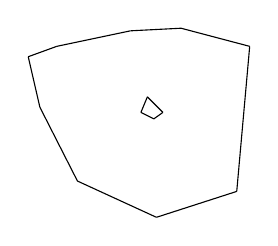
\begin{tikzpicture}
\draw (3.7796,7.1184) -- (4.1414,7.2500);
\draw (5.4079,5.0789) -- (6.4276,5.4079);
\draw (5.0789,7.4474) -- (5.7204,7.4803);
\draw (3.7796,7.1184) -- (3.9276,6.4770);
\draw (5.2105,6.4112) -- (5.3750,6.3289);
\draw (5.7204,7.4803) -- (6.5921,7.2500);
\draw (5.3750,6.3289) -- (5.4901,6.4112);
\draw (4.4046,5.5395) -- (5.4079,5.0789);
\draw (4.1414,7.2500) -- (5.0789,7.4474);
\draw (3.9276,6.4770) -- (4.4046,5.5395);
\draw (6.5921,7.2500) -- (6.4276,5.4079);
\draw (5.2928,6.6086) -- (5.2105,6.4112);
\draw (5.2928,6.6086) -- (5.4901,6.4112);
\fill (3.7796,7.1184) circle;
\fill (4.1414,7.2500) circle;
\fill (5.0789,7.4474) circle;
\fill (5.7204,7.4803) circle;
\fill (6.5921,7.2500) circle;
\fill (3.9276,6.4770) circle;
\fill (4.4046,5.5395) circle;
\fill (5.4079,5.0789) circle;
\fill (6.4276,5.4079) circle;
\fill (5.2928,6.6086) circle;
\fill (5.2105,6.4112) circle;
\fill (5.3750,6.3289) circle;
\fill (5.4901,6.4112) circle;
\end{tikzpicture}
